\chapter{Integrace do průmyslu 4.0}
Pojem Průmysl 4.0 se do České republiky dostal okolo roku 2013 a~od té doby se stále více rozšiřuje v~průmyslových firmách.
Jedna z~klíčových částí je IoT (Internet of Things), neboli internet věcí, který nám zajišťuje vzdálenou kontrolu a~řízení strojů pomocí elektroniky, senzorů a~různých softwarů.
Další vlastností těchto systémů je zaznamenávání a~následné ukládání dat do datových úložišť.
Moderní IoT řídící systémy se snaží proniknou co nejvíce do hloubky a~zpřesnit tak naměřená data, důležitá pro optimalizaci produkce.   

%SECTION
\section{Práce operátorů}
Každá pracovní směna se skládá ze tří operátorů, kdy každý se stará o pět až osm pletacích strojů.
Z každého pletacího stroje vypadne každé čtyři minuty jedna upletené ponožka, kterou operátor musí zkontrolovat a otočit naruby pro další zpracování.
Dalším úkolem operátorů je doplňování materiálu a oprava strojů při poruše.

%SECTION
\section{Popis}
Při~návrhu mého systému jsem se snažil řídit těmito zásadami a~navrhnout tak co nejmodernější a~provozně efektivní systém.
Základem bylo zhodnocení stávající situace a~navržení možného řešení.

Jednotlivé problémy neautomatizované výroby:
\begin{itemize}
    \item dlouhá doba stání nečinných strojů při poruše i nedostatku materiálu
    \item neznalost doby nečinnosti stroje
    \item ruční počítání vyprodukovaného zboží
    \item absence historického přehledu produkce
\end{itemize}

%SECTION
\section{Řešení}
Mým řešením je tedy návrh moderního systému, který by celý tento výrobní provoz monitoroval a~zobrazoval jak operátorovi u stroje, tak zaměstnavateli.
Systém umožňuje on line zhodnocení jednotlivých směn a~jejich vzájemné porovnání.
Systém neustále vyvíjím a~rozšiřuji podle potřeb firmy.

Současné funkce systému Pletačka IoT
\begin{itemize}
    \item monitoring chodu každého pletacího stroje
    \item on-line hlášení závady na stroji
    \item monitoring provozu firmy
    \item porovnání pracovních směn
    \item počítání upletených ponožek
\end{itemize}



%SECTION
\section{Nasazení}
Tento systém je aktuálně nasazen ve firmě ROTEX Vysočina \cite{ROTEX}, která se věnuje výrobě ponožek. 
Firma pracuje ve dvousměnném provozu a~týdně vyprodukuje v~průměru 12000 párů ponožek. 

% Díky mému systému by se ve firmě dala optimalizovat produkce a~výkon strojů a~tím zefektivnit budoucí výrobu. 
Díky mému systému Pletačka IoT se ve firmě optimalizovala produkce a výkon strojů a tím zefektivnila výroba. 
Toto se podařilo především díky minimalizování času nečinnosti pletacích strojů z důvodu on line hlášení poruch a úsporou času operátora výroby při dřívějším ručním počítáním upletených ponožek. 
Jako bonus navíc systém vyhodnocuje produktivitu každého zaměstnance a jednotlivé směny.

\begin{figure}[htbp]
    \centering
    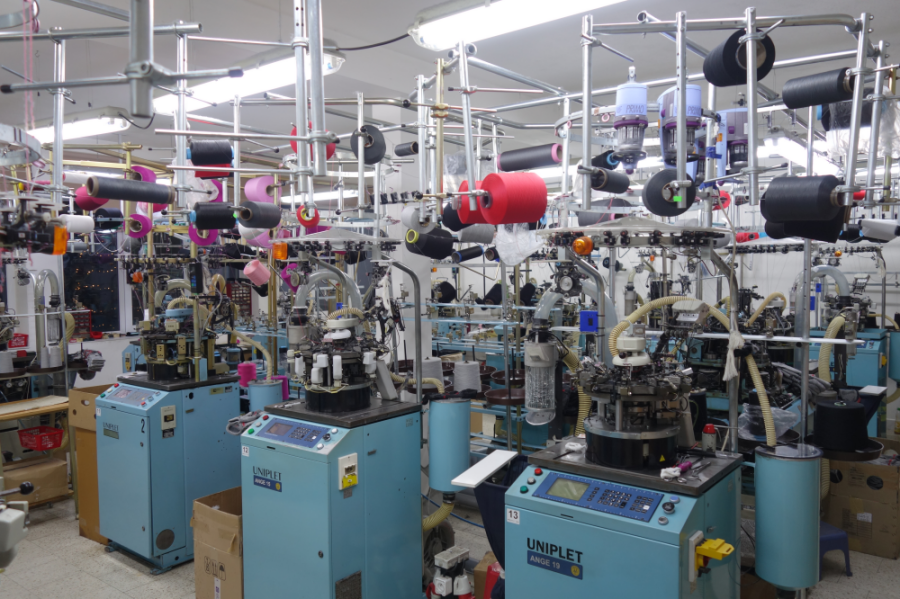
\includegraphics[width=\textwidth]{img/pletarna.png}
    \caption{Pletárna ponožek}
    \label{fig:Pletarna}
\end{figure}

% \begin{figure}[htbp]
%     \centering
%     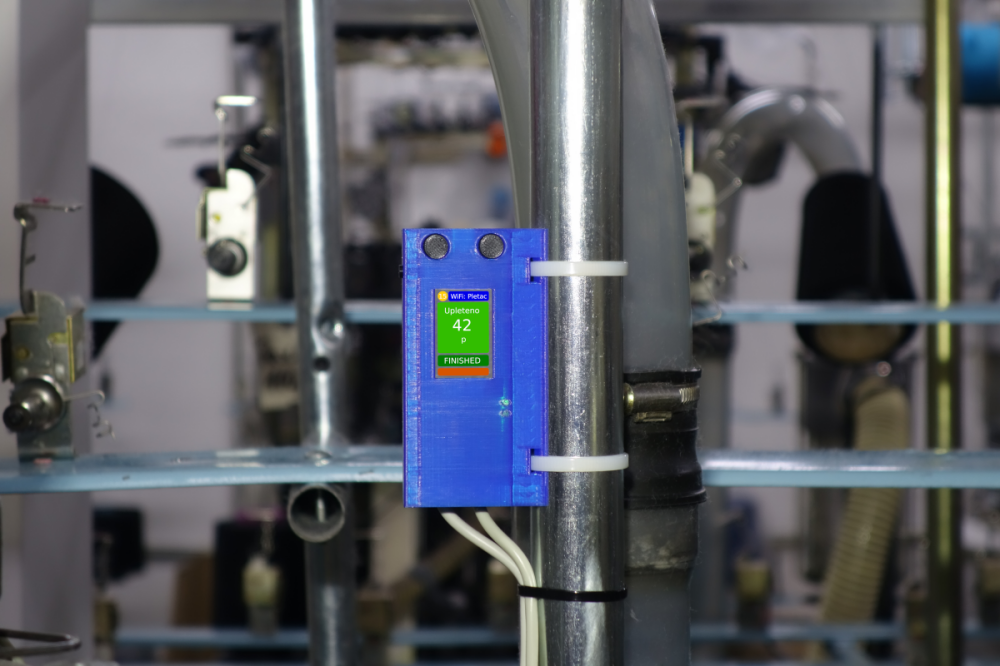
\includegraphics[width=\textwidth]{img/V2-uchyceni.png}
%     \caption{Senzor na stroji}
%     \label{fig:SenzorNaStroji}
% \end{figure}


\newpage
